\documentclass[tikz,border=4pt]{standalone}
\usepackage{amsmath,amssymb}\renewcommand{\familydefault}{\sfdefault}
\usepackage{pgfplots}\pgfplotsset{compat=1.17}
\usetikzlibrary{arrows.meta,positioning,shadows,fit,calc,backgrounds,patterns}
\definecolor{lav}{HTML}{E6E6FF}\definecolor{pinkb}{HTML}{FFDDDD}\definecolor{greenb}{HTML}{DDFFDD}\definecolor{yelb}{HTML}{FFFBCF}\definecolor{peach}{HTML}{FFEBD6}\definecolor{mauve}{HTML}{F0E6F0}
\definecolor{reqblue}{HTML}{0000BB}\definecolor{resgreen}{HTML}{008800}\definecolor{dred}{HTML}{CC0000}\definecolor{domblue}{HTML}{000099}\definecolor{crimson}{HTML}{990033}
\definecolor{tbBlue}{HTML}{1F77B4}\definecolor{tbOrange}{HTML}{FF7F0E}\definecolor{tbGreen}{HTML}{2CA02C}\definecolor{tbRed}{HTML}{D62728}\definecolor{tbPurple}{HTML}{9467BD}\definecolor{tbBrown}{HTML}{8C564B}
\definecolor{barGreen}{HTML}{1B8754}\definecolor{darkGreen}{HTML}{2E7D32}\definecolor{lightBlue}{HTML}{A0C4FF}\definecolor{kRed}{HTML}{DC3545}
\definecolor{accB}{HTML}{3366FF}\definecolor{f1O}{HTML}{FF7F50}\definecolor{aucG}{HTML}{44CC11}
\tikzset{node/.style={draw,rounded corners=2.5pt,thick,align=center},
 req/.style={-{Stealth[length=2.4mm]},thick,reqblue},res/.style={-{Stealth[length=2.4mm]},thick,dashed,resgreen}}
\pgfplotsset{every axis/.append style={tick label style={font=\footnotesize},label style={font=\small},title style={font=\small},legend style={font=\footnotesize,fill=white,fill opacity=.9,text opacity=1,draw=black!25,rounded corners=1pt},
 grid style={dotted,black!35}}}
\begin{document}
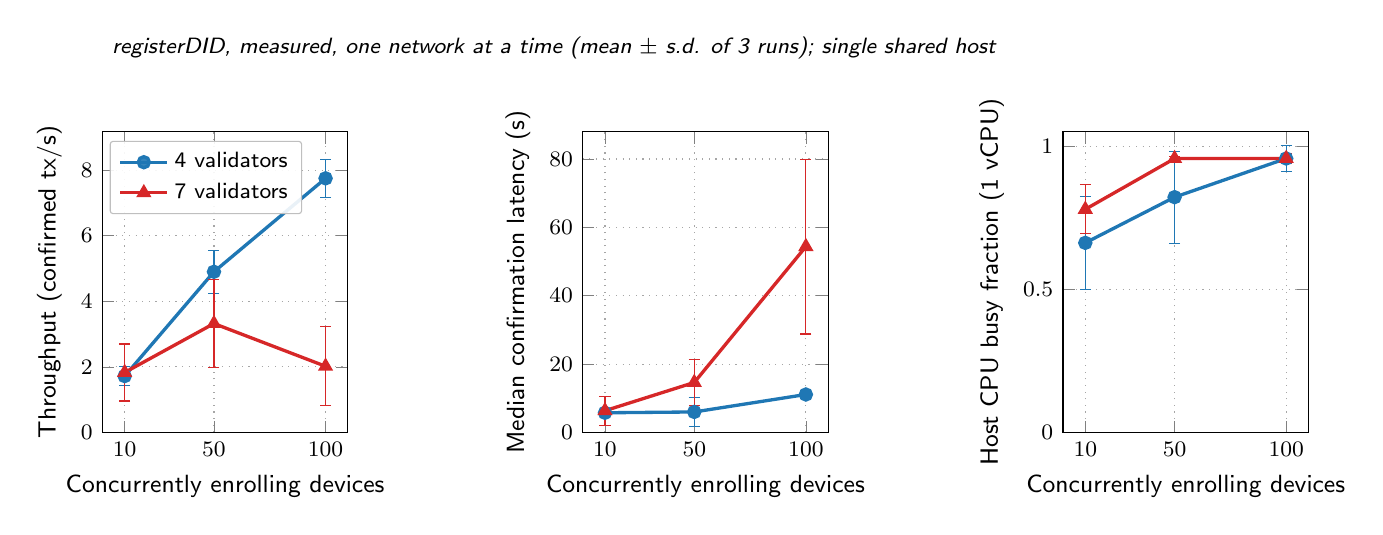
\begin{tikzpicture}
\begin{axis}[at={(0.0cm,0)},anchor=north west,width=4.7cm,height=5.4cm,xmin=0,xmax=110,xtick={10,50,100},xlabel={Concurrently enrolling devices},ylabel={Throughput (confirmed tx/s)},grid=both,ymin=0,legend pos=north west,legend cell align=left]
\addplot[tbBlue,mark=*,line width=1.2pt,error bars/.cd,y dir=both,y explicit] coordinates {(10,1.7192) +- (0,0.29749) (50,4.9015) +- (0,0.65347) (100,7.7513) +- (0,0.58574)}; \addlegendentry{4 validators}
\addplot[tbRed,mark=triangle*,line width=1.2pt,error bars/.cd,y dir=both,y explicit] coordinates {(10,1.8293) +- (0,0.87058) (50,3.3221) +- (0,1.3315) (100,2.0186) +- (0,1.2094)}; \addlegendentry{7 validators}
\end{axis}
\begin{axis}[at={(6.1cm,0)},anchor=north west,width=4.7cm,height=5.4cm,xmin=0,xmax=110,xtick={10,50,100},xlabel={Concurrently enrolling devices},ylabel={Median confirmation latency (s)},grid=both,ymin=0,legend pos=north west,legend cell align=left]
\addplot[tbBlue,mark=*,line width=1.2pt,error bars/.cd,y dir=both,y explicit] coordinates {(10,5.7558) +- (0,0.90463) (50,5.9988) +- (0,4.2004) (100,11.104) +- (0,1.2866)};
\addplot[tbRed,mark=triangle*,line width=1.2pt,error bars/.cd,y dir=both,y explicit] coordinates {(10,6.362) +- (0,4.2454) (50,14.623) +- (0,6.824) (100,54.374) +- (0,25.583)};
\end{axis}
\begin{axis}[at={(12.2cm,0)},anchor=north west,width=4.7cm,height=5.4cm,xmin=0,xmax=110,xtick={10,50,100},xlabel={Concurrently enrolling devices},ylabel={Host CPU busy fraction (1 vCPU)},grid=both,ymin=0,ymax=1.05,legend pos=north west,legend cell align=left]
\addplot[tbBlue,mark=*,line width=1.2pt,error bars/.cd,y dir=both,y explicit] coordinates {(10,0.66214) +- (0,0.16325) (50,0.82174) +- (0,0.1609) (100,0.95679) +- (0,0.045813)};
\addplot[tbRed,mark=triangle*,line width=1.2pt,error bars/.cd,y dir=both,y explicit] coordinates {(10,0.77927) +- (0,0.085326) (50,0.95664) +- (0,0.0062221) (100,0.95683) +- (0,0.017678)};
\end{axis}
\node[font=\footnotesize\itshape,anchor=south west] at (0,0.8) {registerDID, measured, one network at a time (mean $\pm$ s.d. of 3 runs); single shared host};
\end{tikzpicture}
\end{document}
